\documentclass{scrreprt} % comment this out when done editing
% \documentclass{standalone}
% \usepackage{standalone}
\usepackage{chez}

\begin{document}

\section{Can you taste the "diet" in diet soda}

Some people claim that they can tell the difference between a diet soda and a regular soda in the
first sip. A researcher wanting to test this claim randomly sampled 80 such people. He then filled
80 plain white cups with soda, half diet and half regular through random assignment, and asked
each person to take one sip from their cup and identify the soda as diet or regular. Fifty-three
participants correctly identified the soda. Do these data provide strong evidence that these people
are able to detect the difference between diet and regular soda (i.e. that they are doing better
than expected by random guessing)?

\section{State}

We will conduct a 95\% confidence z-test in order to determine whether there
is an observable difference between diet and regular soda.

\section{Plan}

\begin{itemize}
	\item 80 people is less than 10\% of all people.
	\item Let's define $p_c$ as the proportion that correctly identify the soda.
	\item The people who correctly identified the soda are independent of
	the people who did not correctly identify the soda.
	\item Then, $n\hat{p_c}$ is the number of people who correctly identify
	the soda, and $n\hat{p_c} = 53 > 10$.
	\item $n(1-\hat{p_c})$ is the number of people who incorrectly identify the
	soda, and $n(1-\hat{p_c})= 27 > 10$.
\end{itemize}

\section{Do}

% insert image in latex
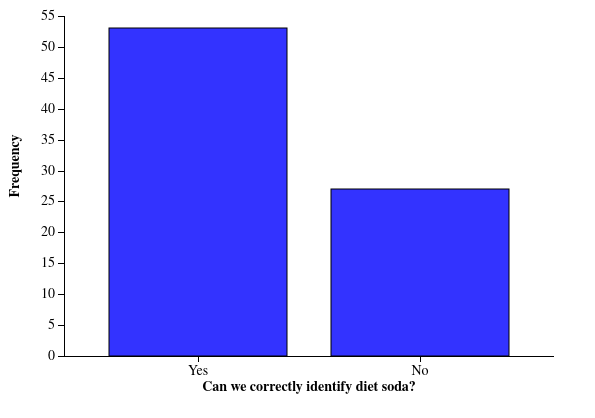
\includegraphics[width=300px]{2021-08-31-11-24-27.png}

\end{document}